%%%%%%%%%%%%%%%%%%%%%%%%%%%%%%%%%%%%%%%%%%%%%%%%%%%%%%%%%%%%%%%%%%%%%%%%%%%%%%%%
% Zynq Platform
%%%%%%%%%%%%%%%%%%%%%%%%%%%%%%%%%%%%%%%%%%%%%%%%%%%%%%%%%%%%%%%%%%%%%%%%%%%%%%%%
\subsection{Zynq Platform}
\begin{frame}[label=zynq]{Zynq Platform}
    \makebox[\textwidth][c]{
        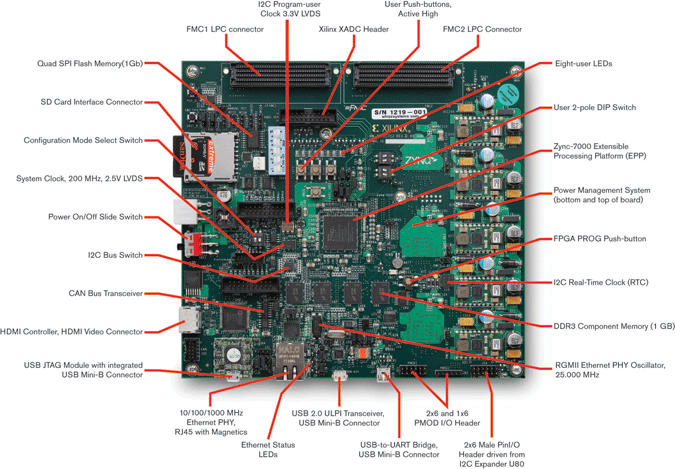
\includegraphics[height=0.88\textheight]{xilinx/zc702-base-board}}
\end{frame}

%%%%%%%%%%%%%%%%%%%%%%%%%%%%%%%%%%%%%%%%%%%%%%%%%%%%%%%%%%%%%%%%%%%%%%%%%%%%%%%%
% Design
%%%%%%%%%%%%%%%%%%%%%%%%%%%%%%%%%%%%%%%%%%%%%%%%%%%%%%%%%%%%%%%%%%%%%%%%%%%%%%%%
% In this section, illustrate the hardware and software interface for the
% design. Note that the most important part of the hardware design is
% parallelism, so it is important to mention how this was achieved.
\subsection{Design}
\begin{frame}[label=design]{Design}
    % Block diagram showing hardware, software and interface
    % Multiple functional units
    % Instruction level parallelism
    % Pipelining
\end{frame}

%%%%%%%%%%%%%%%%%%%%%%%%%%%%%%%%%%%%%%%%%%%%%%%%%%%%%%%%%%%%%%%%%%%%%%%%%%%%%%%%
% Results
%%%%%%%%%%%%%%%%%%%%%%%%%%%%%%%%%%%%%%%%%%%%%%%%%%%%%%%%%%%%%%%%%%%%%%%%%%%%%%%%
\subsection{Results}
\begin{frame}[label=results]{Results}
    % How many cycles the hardware design takes
    % Reference to Amdahl's Law
    % "On this hardware, we expect a speed up of X"
    % Performance estimates
    % Performance comparison
    % Complexity (scaling)
\end{frame}
